\chapter{Introduction}	

% Adpated from: https://www.nasa.gov/reference/appendix-i-verification-and-validation-plan-outline/

\section{Purpose and Scope}

This document describes the testing procedures required to verify and validate the TM Chain developed for SeeSat e.V. within in the Software-Hardware Projekt course. The purpose of the V\&V Plan is to identify the activities that will establish compliance with the requirements (verification) and to establish that the system will meet the customers’ expectations (validation).

\section{Responsibility and Change Authority}

This plan will be maintained by the entire working group, with changes made as they see fit. Changes to the plan after version 1.0 may be made by any individual person of the team, but only after discussing them with the other team members.

\section{Definitions}

%\section{Black Box End to End Validation}

%This document describes an end to end test, as required by SeeSat-WPD-TSL-0004 to show that all incomming data is correctly transmitted.

%\section{White Box Verification}

%Additionally, a full white box verification campaign is described, as the correct implemenatation of the CCSDS' requirements can not be validated by a simple black box test.

\chapter{Applicable and Reference Documents}

\section{Applicable Documents}
\section{Reference Documents}
\begin{itemize}
	\item CCSDS-131.0-B-5
	\item CCSDS-132.0-B-3
	\item AMBA AXI-Stream Protocol Specification
	\item Development Process - HW/SW Projekt TSL - 0004
\end{itemize}
\section{Order of Precendence}

\chapter{System Description}

This chapter describes the system that this plan covers. Its purpose is to give proper context for anybody reading this plan without requiring any further documents. Knowledge of the relevant CCSDS standards is highly beneficial for the reader's understanding of the system.

\section{System Architecture}

The system under test, as pictured in figure \ref{fig:systemArch} aims to implement the TM Space Data Link Protocol layer of CCSDS-132 and the TM Synchronization and Channel Coding layer of CCSDS-131. It is divided into 4 major subsystems, namely one encoder and one decoder for each of the relevant layers. The OnBoard-Computer (OBC) and Ground Support Equipment (GSE) are not within the scope of this system, but may be briefly mentioned, as their interfaces are shared with parts of the system. The communication between the the subsystems is implemented using the AMBA AXI-Stream protocol.

\begin{figure}[hbt]
	\centering
	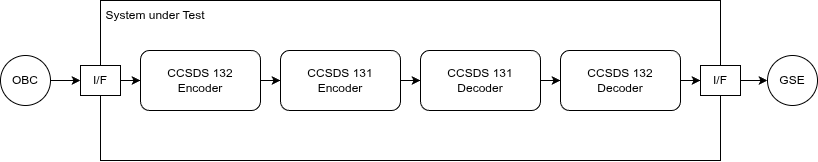
\includegraphics[width=\linewidth]{img/SystemArch.drawio.png}
	\caption{System Architecture}
	\label{fig:systemArch}
\end{figure}

\section{End Item Architectures}

\section{CCSDS 132 Encoder}
\label{sec:ccsds_132_encoder}
\section{CCSDS 131 Encoder}

In general, the CCSDS 131 Encoder can be subdivided into four components defined by CCSDS 131.0-B-5. The first of these is the Reed-Solomon encoder, which is designed to implement a (223, 255)-RS encoder. This means that upto 16-byte errors can be corrected by the code generated here. The R/S encoder reads a one-byte-wide data stream from higher layers and sends a one-byte-wide data stream to lower layers of the CCSDS 131.0-B-5.

The following components, namely the RNG, ASM and CC, require a one-bit-wide datastream. This is why an auxiliary module, the width converter, is introduced. This converts a 8-bit-wide datastream to a one-bit-wide datastream. This module allows a clear separation of concern between the Reed-Solomon encoder and the RNG unit. Neither element requires knowledge of the width of the data stream used in the other layers. This allows for low coupling between these layers and enables components to be changed if required.

The output stream can then be sent to the pseudorandomiser (RNG) module, which implements a linear feedback shift register using a generator polynomial to generate a random sequence. This randomisation is reset with each R/S code word, thus generating the same random sequence for each code word. The random bit value is then added to the one-bit stream received from the R/S encoder and sent to the ASM unit.

The Attached Sync Marker (ASM) module prepends a synchronisation pattern to the data stream generated by the RNG module every R/S code word, allowing the R/S decoder and RNG unit on the receiving side to resynchronise. It then forwards all data generated by the RNG module to the convolutional code (CC) module, along with the added synchronisation patterns.

The CC module implements a convolution over the received datastream from the ASM unit. This convolution is implemented over two different polynomials, thus generating a datastream with a data rate twice that of the input data rate while continuously changing between the two polynomials. The output of this module is the final stage of the 131 encoder and will be sent to the physical layer.

\begin{figure}[hbt]
	\centering
	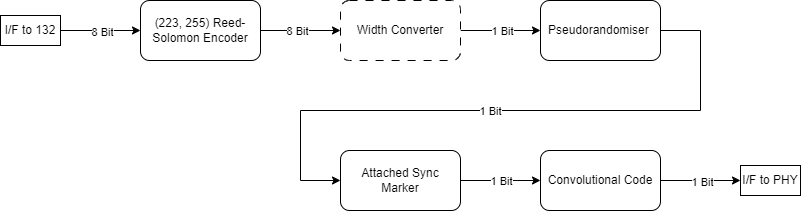
\includegraphics[width=\linewidth]{img/131Encoder.drawio.png}
	\caption{Internal Architecture of the 131 Encoder}
	\label{fig:131Encoder}
\end{figure}

\section{CCSDS 131 Decoder}

Similar to the CCSDS 131 encoder, the decoder can also be divided into four components, as defined by CCSDS 131.0-B-5. The first element is the convolutional decoder. The general goal of this decoder is to recompute the most likely pattern of bits inputted into the CC. In this implementation, this is achieved using a COTS Viterbi decoder. The most probable sequence of bits is then output to the ASM detection unit.

This unit attempts to match the ASM pattern generated by the ASM module on the encoder side with the bitstream generated by the convolutional decoder. This is achieved by calculating the Hamming distance to the expected pattern and triggering an ASM detection if the Hamming distance is lower than a predefined value. Additionally, a counter is implemented to allow for a minimum distance between two detected ASMs, to prevent false detections.

As with the encoder element, the RNG unit generates a randomisation sequence and adds it to the incoming bit stream from the ASM decoder. If an ASM is successfully detected, the RNG unit is reset again to synchronise it with the Reed-Solomon code word. The goal of this unit is to restore the original sequence generated by the Reed-Solomon encoder (including errors not fixed by the Viterbi decoder).

Another auxiliary unit is a second width converter, which converts a one-bit data stream into an eight-bit data stream, thus preparing the data stream for decoding by the R/S decoder.

In contrast to the Viterbi Decoder, the R/S Decoder Unit attempts to find a hard algebraic solution to errors that may have been introduced by the transmission link and not fixed by the Viterbi Decoder. From an architectural point of view, four sub-components are required for this decoder. The first element calculates the syndromes (i.e. the 'illness' of the code), and this information is then forwarded to the next sub-components. This solves the system of equations defined by the syndromes, and finds error locators and error magnitude. These polynomials can then be evaluated by the third sub-component to find the exact error positions and magnitude of the errors. These can then be added to the data stream, which is delayed by the last sub-component. This defines a long FIFO that delays the full data stream for the computational time required by the other three sub-components. The R/S decoder then outputs the corrected datastream and a Reed-Solomon failure flag if decoding failure is detected.

It should be noted that the entire CCSDS 131.0-B-5 decoder outputs a corrupted data stream if the data cannot be corrected; this ensures synchronisation with higher layers.  The R/S Decider is therefore the final element of the CCSDS 131.0-B-5 chain, thereby defining the boundary of this subsystem's system.


\begin{figure}[hbt]
	\centering
	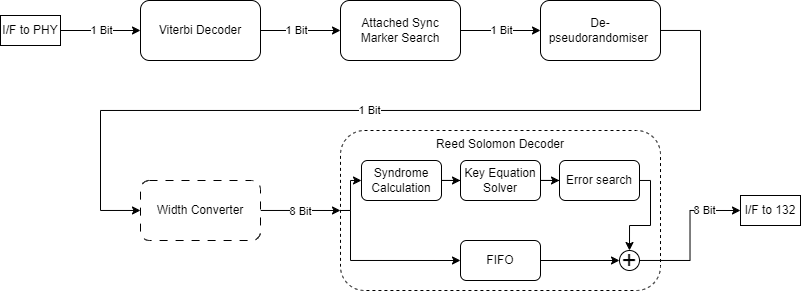
\includegraphics[width=\linewidth]{img/131Decoder.drawio.png}
	\caption{Internal Architecture of the 131 Decoder}
	\label{fig:131Decoder}
\end{figure}

\section{CCSDS 132 Decoder}
The CCSDS 132 Decoder is the ground component of the CCSDS 132-0-b3 Data Link Protocol Sublayer. The decoder is mainly responsible for the extraction of the Space Packets transmitted from on board the satellite. The other data units are not yet implemented and not covered in this document. In order to transmit the Space Packets, the Encoder chain encapsulates them into a TM Transfer frame, from now on called frame. The encoding is described in chapter \ref{sec:ccsds_132_encoder}.

The decoding chain is composed of four stages to demultiplex the different master and virtual channels, indentified by its master channel and virtual channel id, from each other. Figure \ref{fig:132_decoder} shows the data flow of the space packet data from ints source at the 131-decoder to its destination, the AXI 4 Stream FIFO. The complete data flows is positioned in the programmable logic of the SoC with the FIFO as the interface to the processing system. This interface represents the only yet defined service, the packet service.

\begin{figure}[hbt]
	\centering
	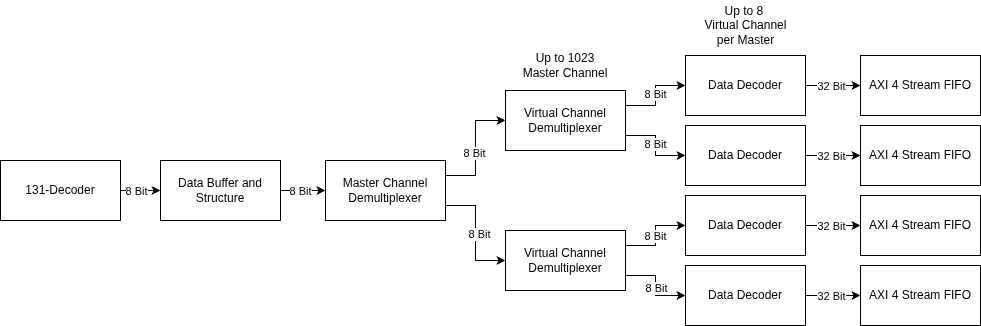
\includegraphics[width=\linewidth]{img/132_decoder.drawio.png}
	\caption{Internal Architecture of 132 Decoder}
	\label{fig:132_decoder}
\end{figure}

The Data Buffer and Structure entity recieves the frame from the 131 decoder in octets, because the frame itself is octet aligned. The purpose of this entity is to buffer the entire frame, decode the header and forward the data field to the master channel demultiplexer. In adition it will delete all only idle data frames.

The master channel demultiplexer routes the data accourding to the provided master channel id to a specified virtual channel demultiplexer. There is one master channel demultiplexer per physical channel. The cahnnel organisation itself is specified by the user and therefore customizable.

The virtual channel demultiplexer routes the data to its designated virtual channel identified by the virtual channel id. There is one instanstance per master channel.

The data decoder recieves the data octets per virtual channel and buffers them once again to decode the space packet header and to check wether the packet is complete. Idle packets and incomplete packets are discarded. In addition to the data, the first header pointer is provided to recieve packets that span over multiple frames. If there is a missmatch between remaining packet data and first header pointer, the partly receive packet will be discarded as well and the first header pointer defines the start of the next valid packet header. The output interface is a 32Bit AXI 4 stream interface. Because of the 8Bit to 32Bit conversion, it is possible, that the output 32Bit will not be filled completely and up to 3 octets will remain in the data decoder until new data is provided at the sending end.

\section{Test Equipment}
Test Equipment is equipment not required by any of the system's requirements, but rather necessary for any of the tests described in this plan. It consists of three important components: the external interface, the Data Generator and the Data Comparator.

\subsection{External Interface}

The external interface connects the other components, which are implemented in the programmable logic part of the SoC to the ethernet interface implemented in the processing system. Through this external interface the test data may be injected into the Data Generator and the output of the Data Comparator is being reported to a connected computer. For interfacing between PL and PS the AXI-4 (lite) protocol is used.

\subsection{Data Generator}

The Data Generator allows the Testsystem to input data into the TM chain. Is uses the CCSDS 132 Encoder's native interface and simulates a connected On-Board Computer by providing valid Space Packets to be sent through the TM chain.

\subsection{Data Comparator}

The Data Comparator receives the data output by the CCSDS 132 Decoder and compares it with the delayed output of the Data Generator. If the output of the decoder matches the expected output, this is reported to the external interface. If they don't match, a bitwise difference is reported for debugging purposes.